\subsection{課題8}
ブラウン運動をコンピュータでシミュレーションしてみる。
\begin{equation}\label{eq:brownian-motion-diff-eq}
    m \odv{\bm{v}}{t} = -\alpha \bm{v} + \bm{f}
\end{equation}
これをコンピュータで解くために差分方程式化すると、
\begin{align}\label{eq:brownian-motion-diff-eq-diff}
    m \dfrac{\bm{v}_{i+1} - \bm{v}_i}{\Delta t} & = -\alpha \bm{v}_i + \bm{f} \nonumber                                                 \\
    \bm{v}_{i+1}                                & = \left( 1 - \dfrac{\alpha \Delta t}{m} \right) \bm{v}_i + \dfrac{\bm{f} \Delta t}{m}
\end{align}
となる。
よって、
\begin{align}\label{eq:brownian-motion-diff-eq-diff-sum}
    \bm{v}_{i} & = \left(1 - \dfrac{\alpha \Delta t}{m}\right)^n \bm{v}_0 + \dfrac{\Delta t}{m} \sum_{i=0}^{n-1} \left(1 - \dfrac{\alpha \Delta t}{m}\right)^i \bm{f}_i
\end{align}
となる。

今、簡単のために$x$のみを考え、粒子の平均速度は0が期待されるから、$\ev{v} = 0$で
$\ev{(v - \ev{v})^2} = \ev{v^2}$である。
多くの粒子についての分散として、$\ev{(v - \ev{v})} = \ev{v^2} - \ev{v}^2$を計算すると、
\begin{align*}
    \ev{v^2} = \left(1 - \dfrac{\alpha \Delta t}{m}\right)^{2n} \ev{(v_0 - \ev{v_0})^2} + \left(\dfrac{\Delta t}{m}\right)^2 \sum_{i=0}^{n-1} \left(1 - \dfrac{\alpha \Delta t}{m}\right)^{2i} \ev{(f_i - \ev{f_i})^2}
\end{align*}
$\ev{(f_i - \ev{f_i})^2}$は、$f$が同一の確率分布に従うとき、
$\ev{(f_i - \ev{f_i})^2} = \ev{(f - \ev{f})^2}$として、
\begin{align*}
    \ev{v^2} & = \left(1 - \dfrac{\alpha \Delta t}{m}\right)^{2n} \ev{(v_0 - \ev{v_0})^2} + \left(\dfrac{\Delta t}{m}\right)^2 \ev{(f - \ev{f})^2} \sum_{i=0}^{n-1} \left(1 - \dfrac{\alpha \Delta t}{m}\right)^{2i} \nonumber                                         \\
             & = \left(1 - \dfrac{\alpha \Delta t}{m}\right)^{2n} \ev{(v_0 - \ev{v_0})^2} + \left(\dfrac{\Delta t}{m}\right)^2 \ev{(f - \ev{f})^2} \dfrac{1 - \left(1 - \dfrac{\alpha \Delta t}{m}\right)^{2(n-1)}}{1 - \left(1 - \dfrac{\alpha \Delta t}{m}\right)^2}
\end{align*}
ここで、$\Delta t$を十分小さくとり、$n \to \infty$とすると、
\begin{align}
    \ev{v^2} & = \left(\dfrac{\Delta t}{m}\right)^2 \ev{(f - \ev{f})^2} \dfrac{1}{1 - \left(1 - \dfrac{\alpha \Delta t}{m}\right)^2} \nonumber \\
             & \approx \dfrac{\Delta t}{2 \alpha m} \ev{(f - \ev{f})^2}
\end{align}
を得る。
気体分子運動論から、$\ev{v^2} = kT/m$であるから、
\begin{equation}
    \ev{(f - \ev{f})^2} = \dfrac{2 \alpha kT}{\Delta t}
\end{equation}
よって、この分散をもつ正規分布に従う乱数を生成し、
\begin{equation}
    x_n = x_{n-1} + v_{n-1} \Delta t
\end{equation}
で位置を計算すればよい。

このシミュレーションを行った結果を図\ref{fig:brownian-2d-sim}に示す。
\begin{figure}
    \centering
    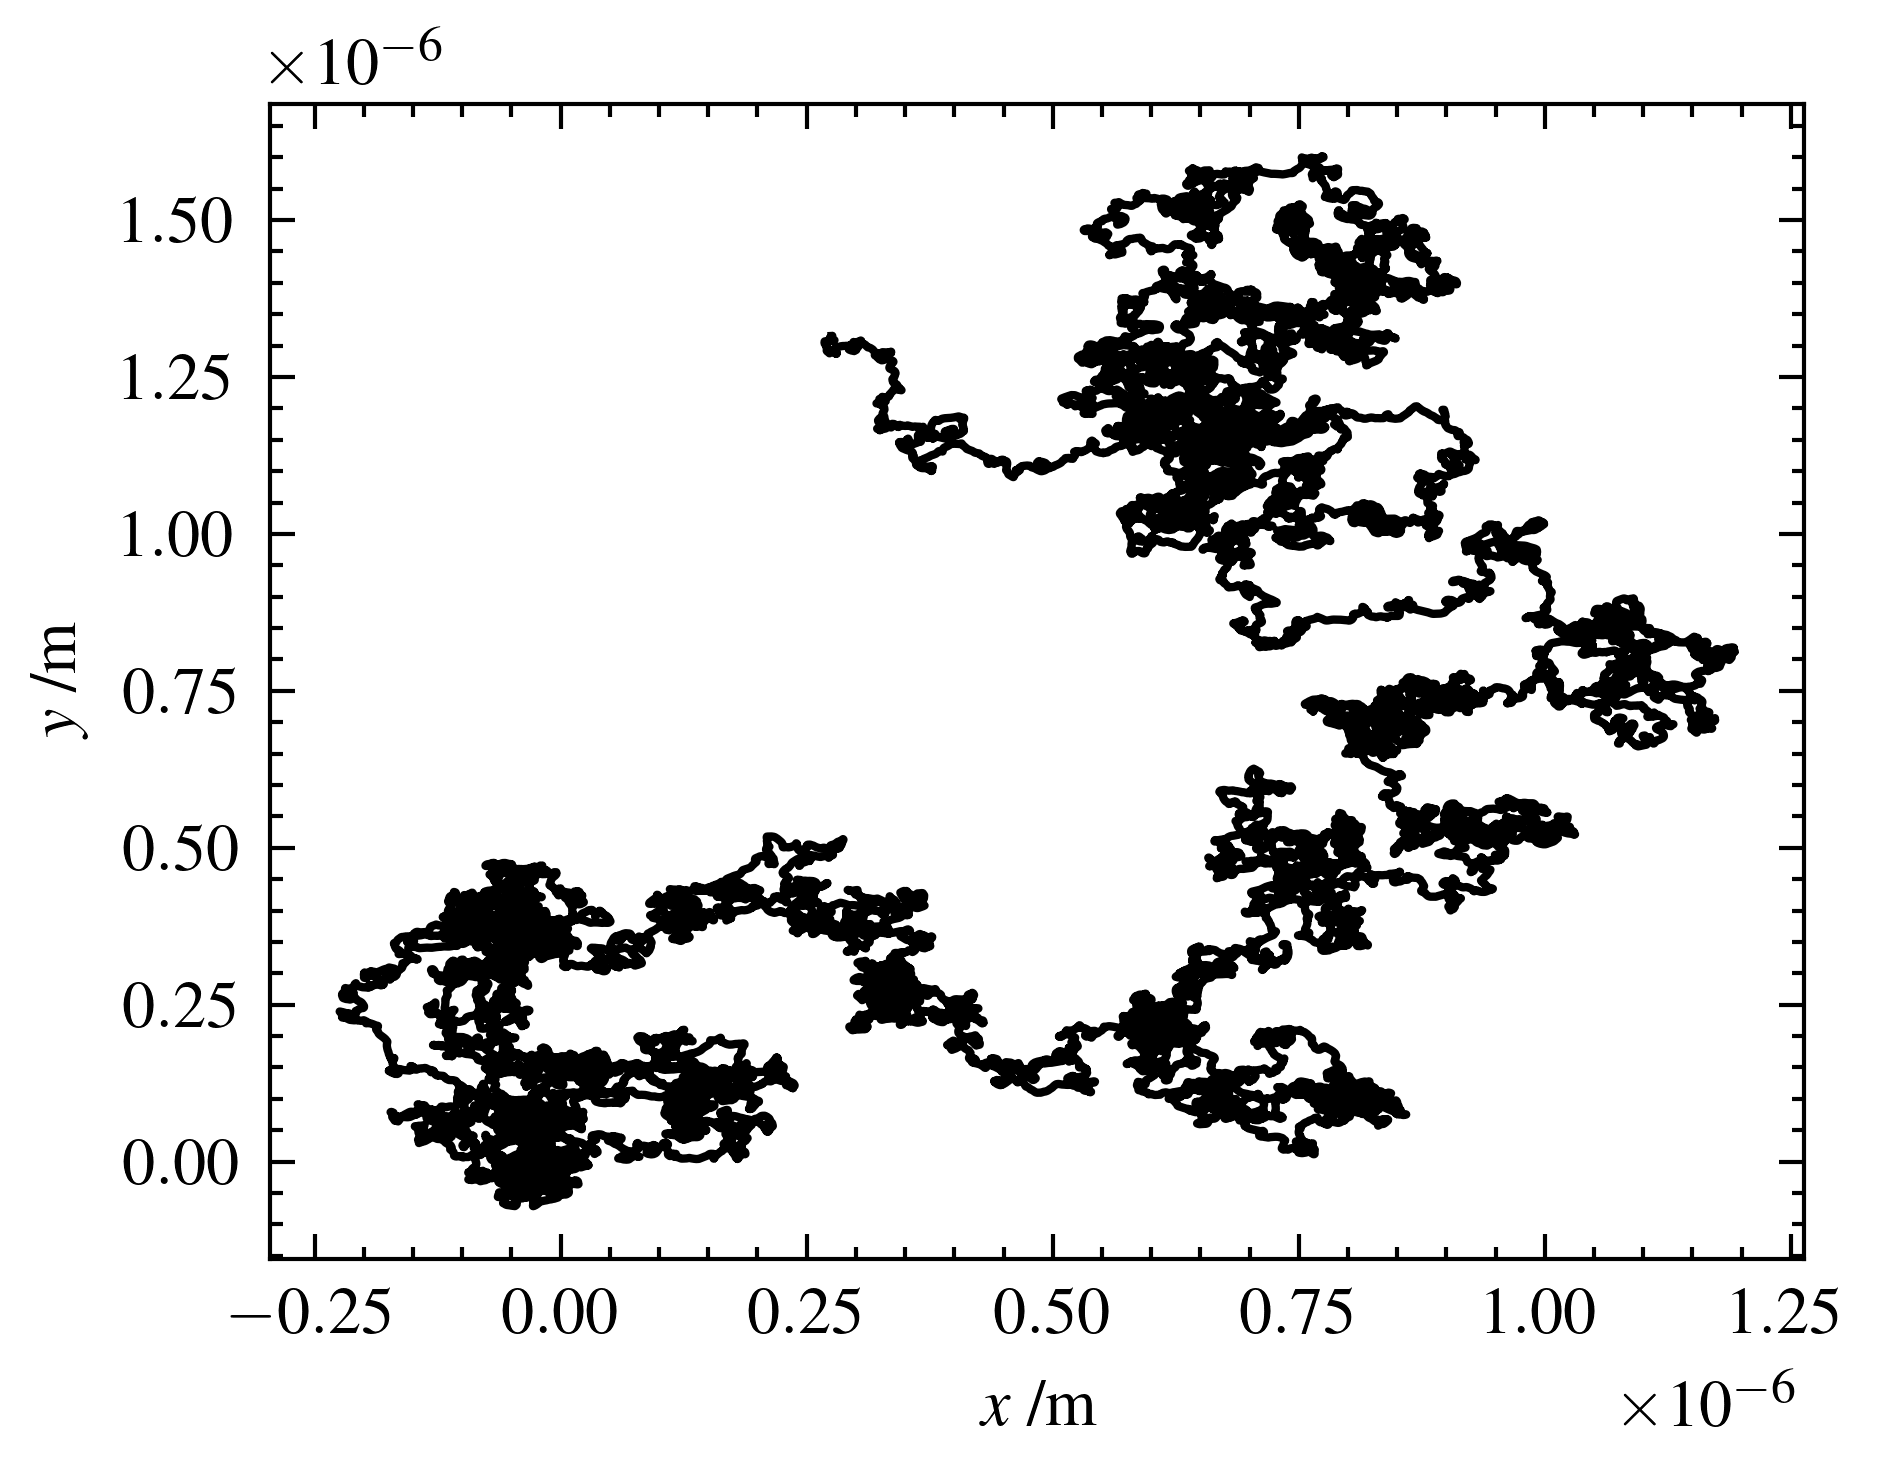
\includegraphics[width=0.8\linewidth]{./src/figures/brownian-2d-sim/brownian-2d-sim.png}
    \caption{2次元ブラウン運動のシミュレーション}\label{fig:brownian-2d-sim}
\end{figure}

この図を見ると、光学顕微鏡で見れる\si{\micro\meter}のオーダーで、
ランダムに動く粒子の動きが再現できている。
